\documentclass[bigger]{beamer}

\usepackage{booktabs}
\useinnertheme{rounded}
\usecolortheme{crane}
\setbeamerfont{block title}{size={}}

\title{Impact of Data Collection on Interpretation and Evaluation of Student
  Models}

\author{\textbf{Radek Pel\'anek}, Ji\v{r}\'i \v{R}ih\'ak, Jan Papou\v{s}ek\\[10mm]
%Masaryk University Brno\\
%Czech Republic

\includegraphics[width=.3\linewidth]{al-logo}
}

\date{LAK 2016}
 
\begin{document}

\frame{\titlepage}

\begin{frame}
  \begin{center}
    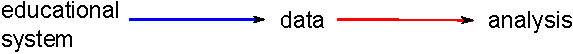
\includegraphics[width=\linewidth]{intro1}
  \end{center}
\end{frame}

\begin{frame}
  \begin{center}
    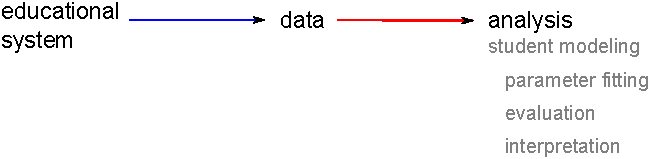
\includegraphics[width=\linewidth]{intro2}
  \end{center}
\end{frame}

\begin{frame}
  \begin{center}
    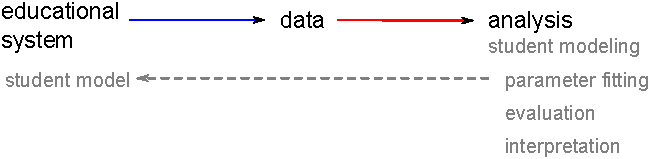
\includegraphics[width=\linewidth]{intro3}
  \end{center}
\end{frame}

\begin{frame}
  \frametitle{Note on Student Models}

  \begin{center}
    \begin{tabular}{ll}
 \textbf{BKT} & Bayesian Knowledge Tracing \\[3mm]
 \textbf{PFA} & Performance Factor Analysis \\[3mm]
 \textbf{Elo} & modified Elo Rating System  \\    
    \end{tabular}
  \end{center}
\end{frame}

\begin{frame}
  \frametitle{Our Focus}

  Issues explored:
  \begin{itemize}
  \item mastery attrition, number of answers per student
  \item item ordering and selection
  \end{itemize}

  \bigskip

  Methods used:
  \begin{itemize}
  \item simulated data
  \item real data (adaptive practice of geography)
  \end{itemize}
\end{frame}

\begin{frame}
  \frametitle{Full Data}
  \begin{center}
    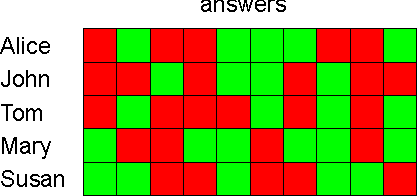
\includegraphics[width=.8\linewidth]{answers-full}
  \end{center}
\end{frame}

\begin{frame}
  \frametitle{Different Number of Answers}
  \begin{center}
    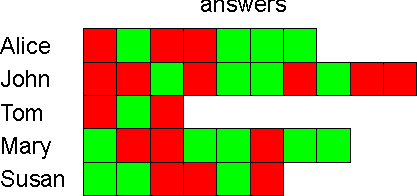
\includegraphics[width=.8\linewidth]{answers-random}
  \end{center}
\end{frame}

\begin{frame}
  \frametitle{Mastery Learning}
  \begin{center}
    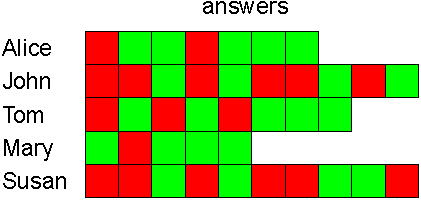
\includegraphics[width=.8\linewidth]{answers-mastery}
  \end{center}
\end{frame}

\begin{frame}
  \frametitle{Mastery Attrition}
  \begin{center}
    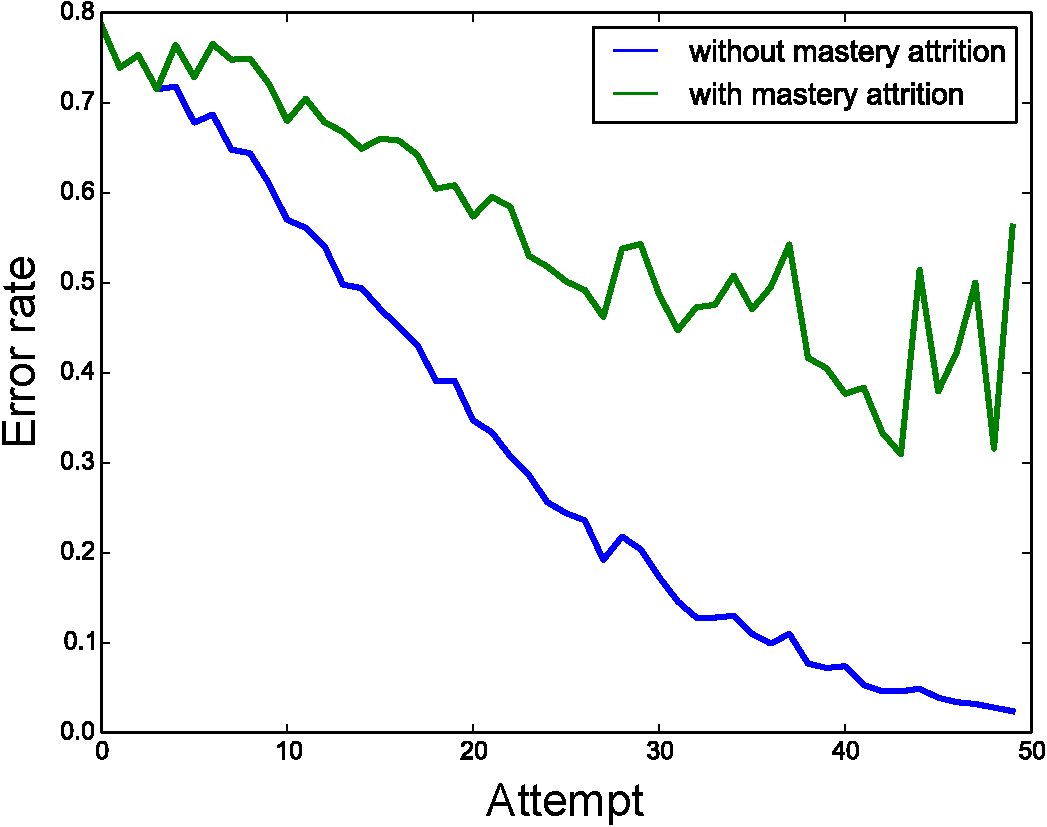
\includegraphics[width=.75\linewidth]{demo-mastery-attrition}
  \end{center}
\end{frame}

\begin{frame}
  \frametitle{Number of Answers -- Impact on Parameter Fitting}
  
  % \begin{itemize}
  % \item data generated by BKT model
  % \item data fitted by PFA model
  % \item fitted parameter values depend the number of answers used 
  % \end{itemize}
  
  \begin{center}
    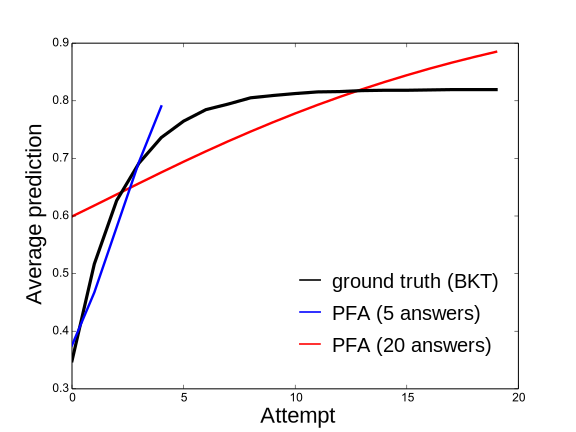
\includegraphics[width=.75\linewidth]{B1-PFA-trace-lengths}
  \end{center}
\end{frame}

\newcommand{\pinit}{P_\mathit{init}}
\newcommand{\plearn}{P_\mathit{learn}}
\newcommand{\pguess}{P_\mathit{guess}}
\newcommand{\pslip}{P_\mathit{slip}}

\begin{frame}
  \frametitle{Parameter Fitting and Mastery Attrition}

  data generated and fitted by BKT model

  \bigskip

  \begin{center}
    \begin{tabular}{lrrrr}
      \toprule
      model & $\pinit$ & $\plearn$ & $\pslip$ & $\pguess$ \\
      \midrule
      ground truth & 0.25 & 0.08 & 0.12 & 0.30 \\
      fitted model (20 answers) & 0.27 & 0.08 & 0.10 & 0.27 \\
      fitted model (mastery learning) &  0.72 & 0.23 & 0.52 & 0.15 \\
      \bottomrule   
    \end{tabular}
  \end{center}
\end{frame}

\begin{frame}
  \frametitle{Mastery Attrition and Model Comparison}
  
  data generated using the logistic function:\\
  $\sigma(\theta + k\cdot 0.1)$, where $\theta \sim \mathcal{N}(-0.4,2)$

  \bigskip
  \bigskip

  \begin{tabular}{lcl}
     constant number of answer & ~~ & PFA better than BKT \\
     mastery learning & ~~ & BKT better than PFA
  \end{tabular}
\end{frame}

\begin{frame}
  \frametitle{Main Message}

  \begin{block}{}
    ``data collection'' may influence results more than ``modeling''    
  \end{block}
\end{frame}

\begin{frame}
  \frametitle{Adaptive Choice of Items}
  
  \begin{itemize}
  \item adaptivity, personalization
  \item select items of appropriate difficulty 
    \begin{itemize}
    \item 75 \% chance of correct answer
    \end{itemize}
  %\item impact on evaluation
  \end{itemize}
\end{frame}

% \begin{frame}
%  \frametitle{Item Ordering}

%   items in increasing difficulty

%   student learning

%   cannot distinguish... 
% \end{frame}

\begin{frame}
   \begin{center}
    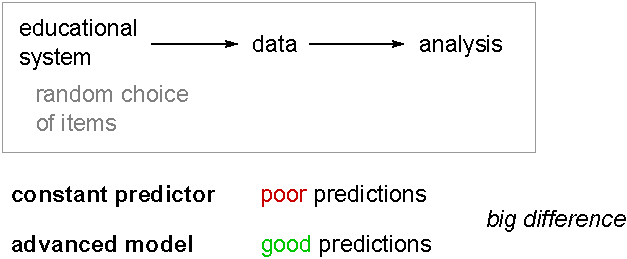
\includegraphics[width=\linewidth]{intro-models1}
   \end{center}
\end{frame}

\begin{frame}
   \begin{center}
    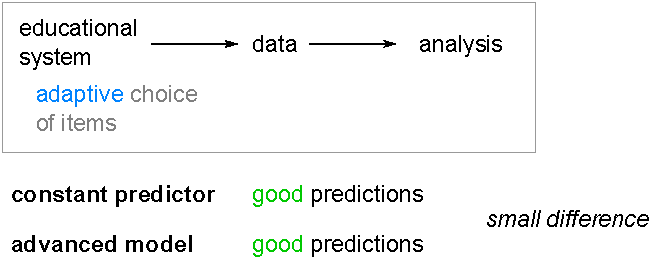
\includegraphics[width=\linewidth]{intro-models2}
   \end{center}
\end{frame}

\begin{frame}
  \frametitle{Data from Experiment}

  \begin{center}
    \texttt{outlinemaps.org}
    \medskip

    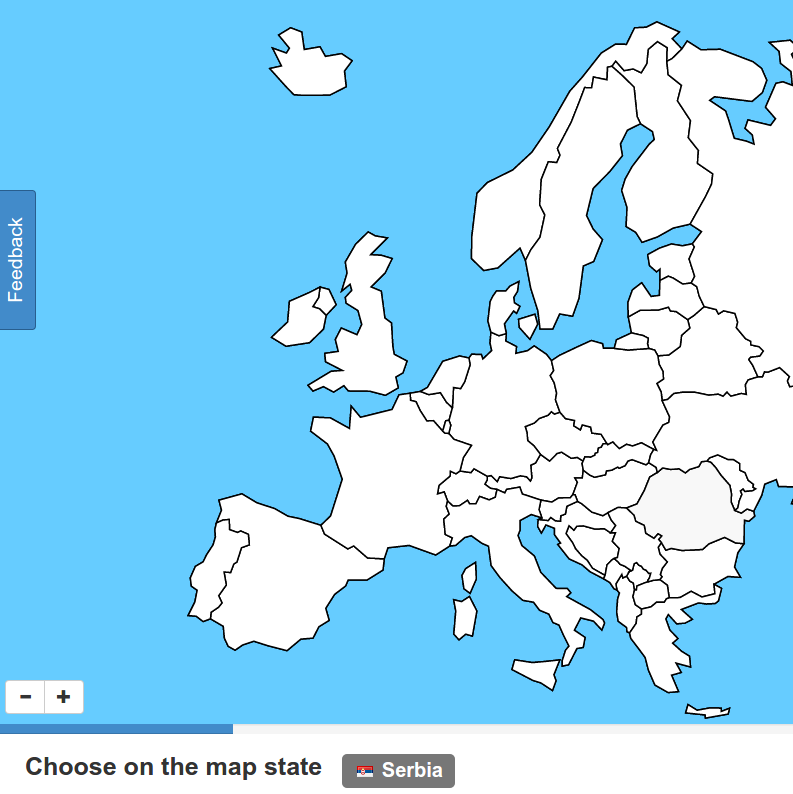
\includegraphics[width=.35\linewidth]{slepemapy-screenshot1}
  \end{center}

  \bigskip 

  randomized trial, comparison of adaptive vs random choice of items\\

  {\footnotesize \emph{Evaluation of an Adaptive Practice System for Learning
      Geography Facts}}
\end{frame}

\begin{frame}
  \frametitle{Impact on Model Evaluation}
  \begin{center}
    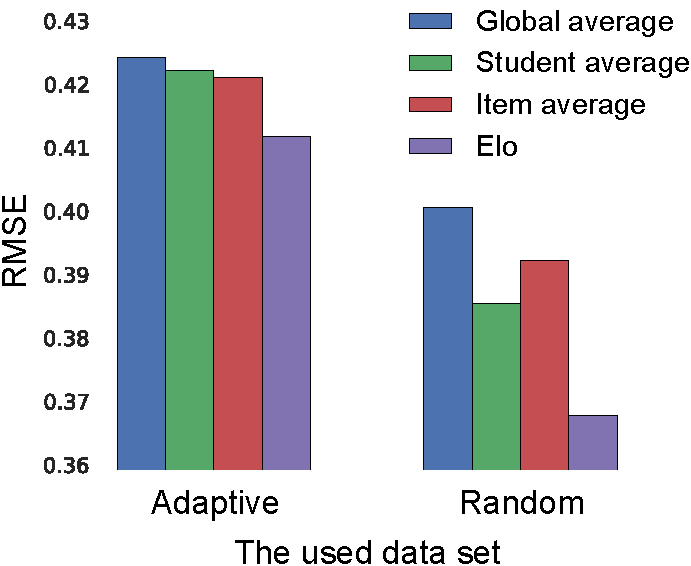
\includegraphics[width=.7\linewidth]{AB-groups-vs-models0}
  \end{center}
\end{frame}

% \begin{frame}
%   \frametitle{Impact on Model Evaluation}
%   \begin{center}
%     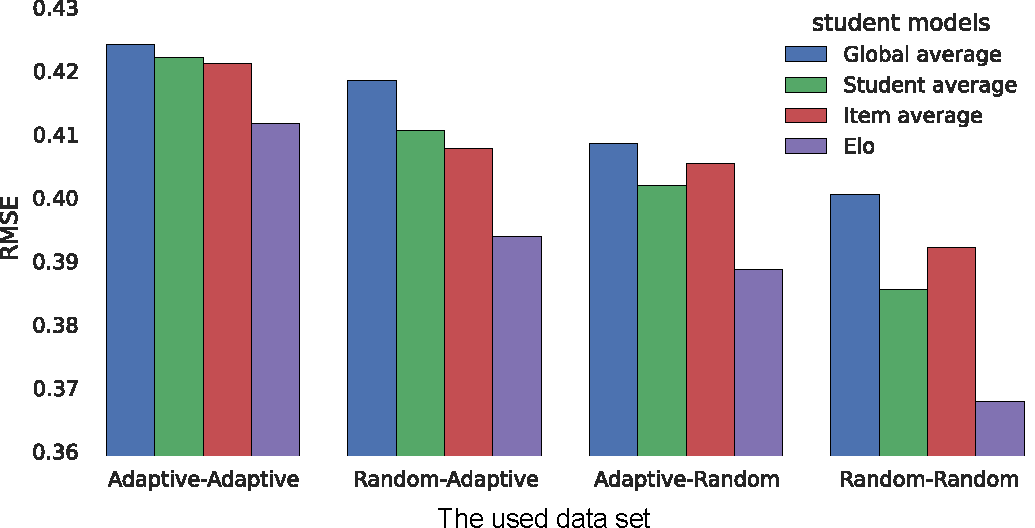
\includegraphics[width=\linewidth]{AB-groups-vs-models}
%   \end{center}
% \end{frame}

\begin{frame}
  \frametitle{Feedback Loop}

  \begin{center}
    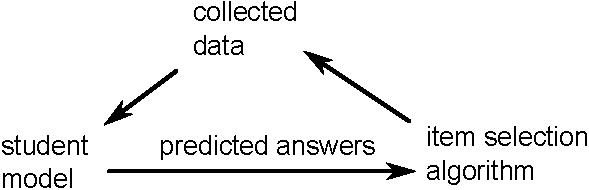
\includegraphics[width=.75\linewidth]{feedback}
  \end{center}
\end{frame}

\begin{frame}
  \frametitle{Feedback Impact}
  \begin{center}
    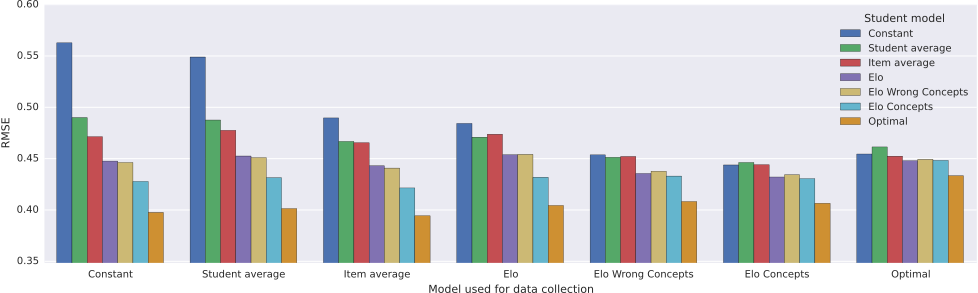
\includegraphics[width=\linewidth]{rmse_complex}
  \end{center}
\end{frame}

\begin{frame}
  \frametitle{Feedback Impact}
  \begin{center}
    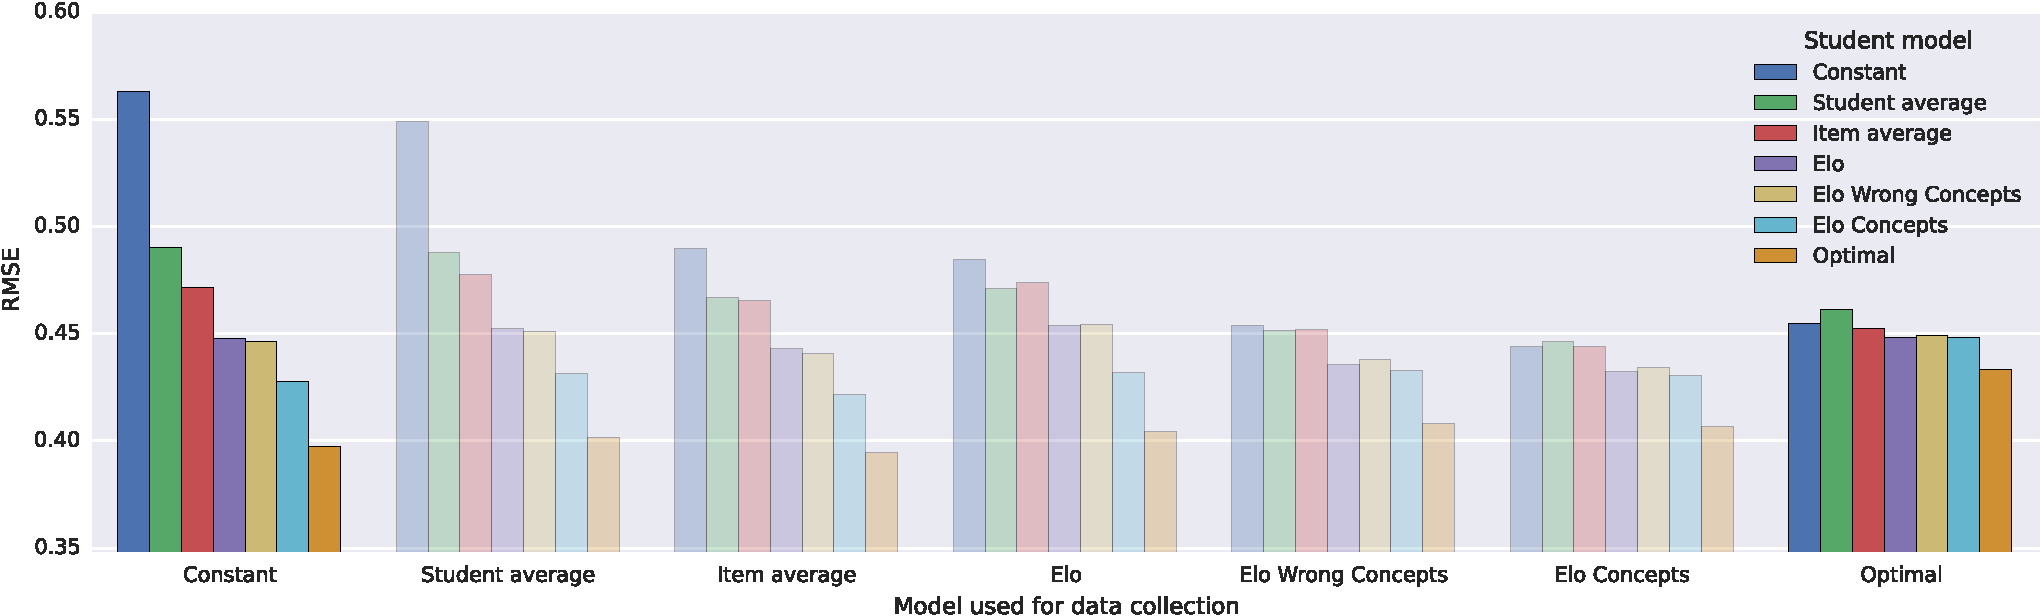
\includegraphics[width=\linewidth]{rmse_complex1}
  \end{center}

  \bigskip

  \begin{center}
    good adaptive educational systems 
    
    $\Downarrow$

    small differences in predictive accuracy\\
    of widely different models
  \end{center}
\end{frame}

\begin{frame}
  \frametitle{Feedback Impact}
  \begin{center}
    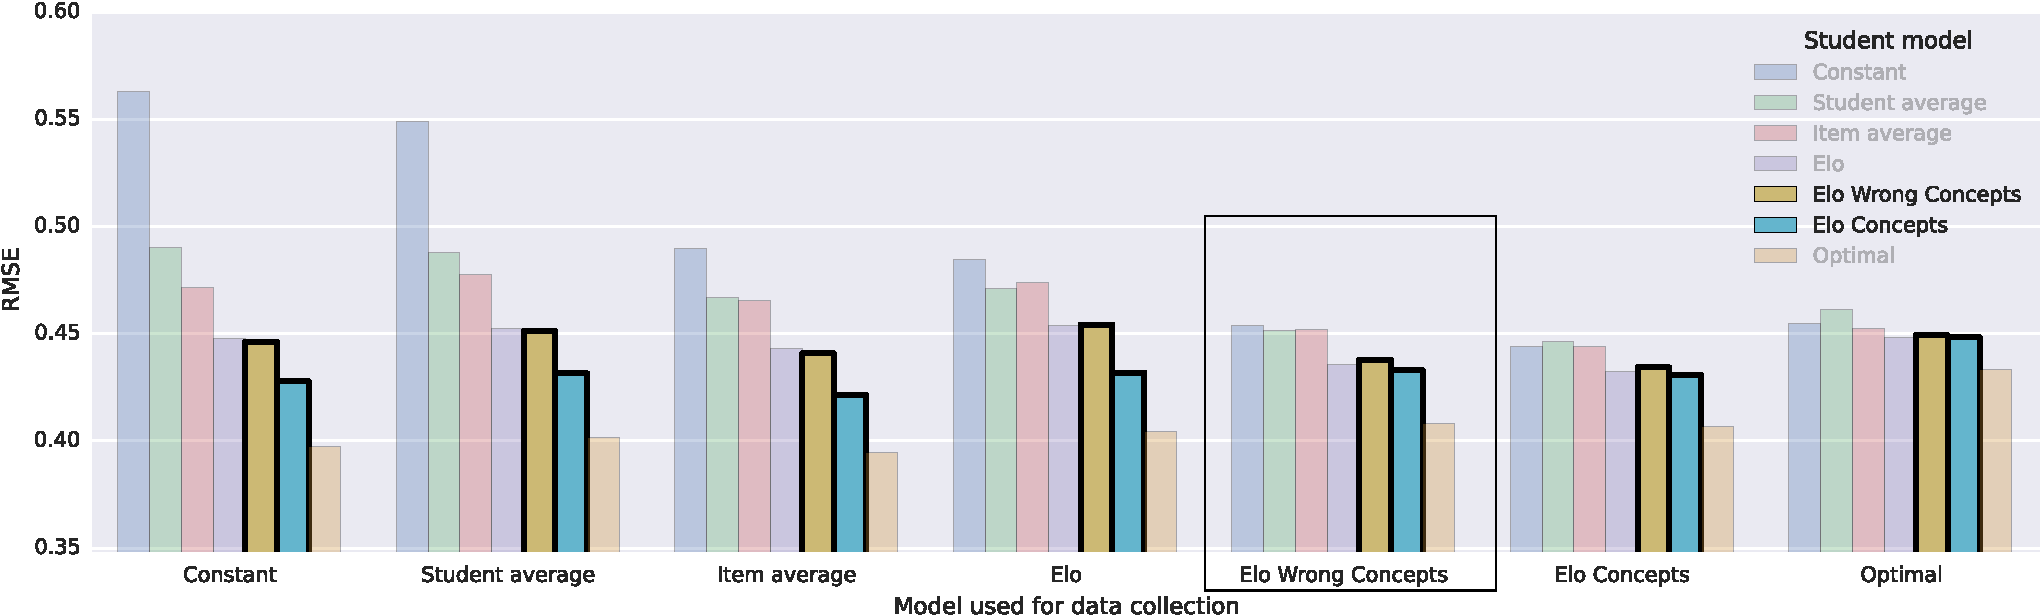
\includegraphics[width=\linewidth]{rmse_complex2}
  \end{center}

  \bigskip

  \begin{center}
    wrong model used in adaptive educational systems 
    
    $\Downarrow$

    collected data insufficient to show deficiencies 
  \end{center}
\end{frame}

\begin{frame}
  \frametitle{Parameter Estimation}

  impact of adaptive choice of items on estimation of item difficulty

  \begin{itemize}
  \item two data collection methods:
    \begin{itemize}
    \item random
    \item adaptive
    \end{itemize}
  \item two estimation methods:
    \begin{itemize}
    \item naive -- percent correct
    \item student model -- Elo 
    \end{itemize}
  \end{itemize}
\end{frame}

\begin{frame}
  \frametitle{Parameter Estimation}
  \begin{center}
    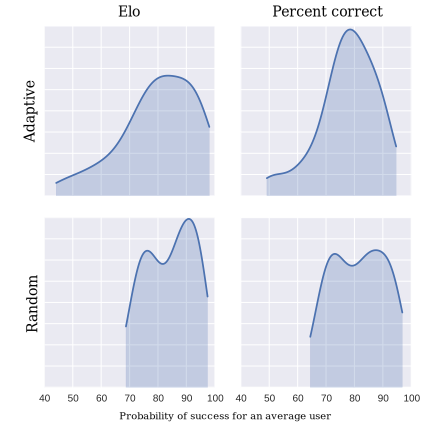
\includegraphics[width=.6\linewidth]{diffs-hist-europe-split}
  \end{center}
\end{frame}

\begin{frame}
  \frametitle{Data Collection Matters}

  data collection influences:
  \begin{itemize}
  \item evaluation of models
    \begin{itemize}
    \item size of differences in comparison metrics
    \item sometimes even ordering of models
    \end{itemize}
  \item interpretation of models
    \begin{itemize}
    \item fitted parameter values
    \item ``discovery with models''
    \end{itemize}
  \end{itemize}
\end{frame}


\begin{frame}
  \frametitle{Consequences for Practice}

  \begin{enumerate}
  \item publication of data sets
    \begin{itemize}
    \item describe data collection mechanism
    \end{itemize}
  \item evaluation and interpretation of models
    \begin{itemize}
    \item understanding of data 
    \item stability of results
    \end{itemize}
  \item data collection
    \begin{itemize}
    \item controlled use of randomization
    \end{itemize}
  \end{enumerate}
\end{frame}

\begin{frame}
  \frametitle{Questions}

  \begin{itemize}
  \item What about your data?
  \item How were they collected?
  \item Does it matter? Does it influence your results?
  \item Are you sure there is no bias?
  \end{itemize}

\end{frame}

% \begin{frame}
%   \frametitle{}
%   \begin{center}
%    \includegraphics[width=\linewidth]{}
%   \end{center}
% \end{frame}

% \begin{frame}
%   \frametitle{}
% \end{frame}



\end{document}